% Created by tikzDevice version 0.10.1 on 2017-05-13 00:07:44
% !TEX encoding = UTF-8 Unicode
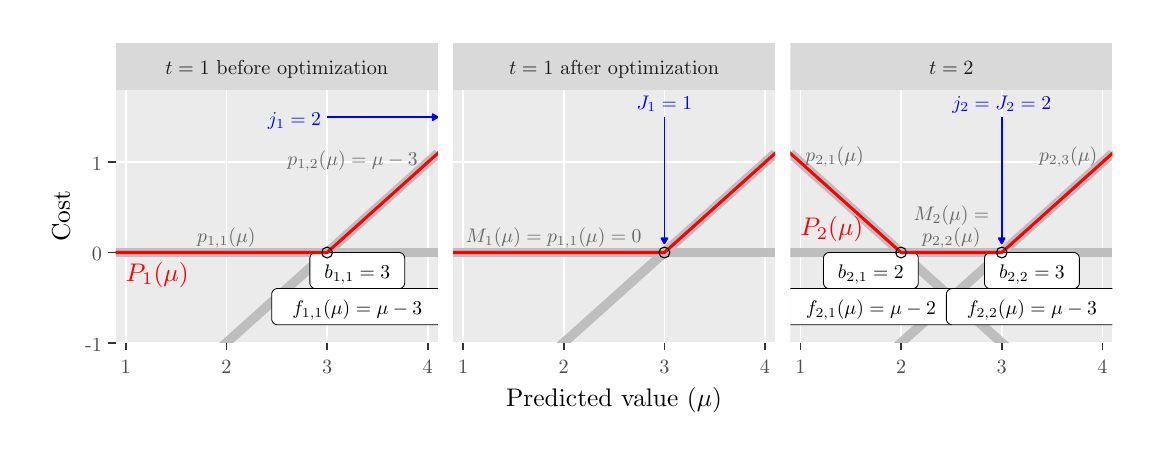
\begin{tikzpicture}[x=1pt,y=1pt]
\definecolor{fillColor}{RGB}{255,255,255}
\path[use as bounding box,fill=fillColor,fill opacity=0.00] (0,0) rectangle (397.48,144.54);
\begin{scope}
\path[clip] (  0.00,  0.00) rectangle (397.48,144.54);
\definecolor{drawColor}{RGB}{255,255,255}
\definecolor{fillColor}{RGB}{255,255,255}

\path[draw=drawColor,line width= 0.6pt,line join=round,line cap=round,fill=fillColor] (  0.00,  0.00) rectangle (397.48,144.54);
\end{scope}
\begin{scope}
\path[clip] ( 31.80,121.98) rectangle (148.20,139.04);
\definecolor{fillColor}{gray}{0.85}

\path[fill=fillColor] ( 31.80,121.98) rectangle (148.20,139.04);
\definecolor{drawColor}{gray}{0.10}

\node[text=drawColor,anchor=base,inner sep=0pt, outer sep=0pt, scale=  0.73] at ( 90.00,127.48) {$t=1$ before optimization};
\end{scope}
\begin{scope}
\path[clip] (153.70,121.98) rectangle (270.09,139.04);
\definecolor{fillColor}{gray}{0.85}

\path[fill=fillColor] (153.70,121.98) rectangle (270.09,139.04);
\definecolor{drawColor}{gray}{0.10}

\node[text=drawColor,anchor=base,inner sep=0pt, outer sep=0pt, scale=  0.73] at (211.89,127.48) {$t=1$ after optimization};
\end{scope}
\begin{scope}
\path[clip] (275.59,121.98) rectangle (391.98,139.04);
\definecolor{fillColor}{gray}{0.85}

\path[fill=fillColor] (275.59,121.98) rectangle (391.98,139.04);
\definecolor{drawColor}{gray}{0.10}

\node[text=drawColor,anchor=base,inner sep=0pt, outer sep=0pt, scale=  0.73] at (333.79,127.48) {$t=2$};
\end{scope}
\begin{scope}
\path[clip] ( 31.80, 30.69) rectangle (148.20,121.98);
\definecolor{fillColor}{gray}{0.92}

\path[fill=fillColor] ( 31.80, 30.69) rectangle (148.20,121.98);
\definecolor{drawColor}{RGB}{255,255,255}

\path[draw=drawColor,line width= 0.6pt,line join=round] ( 31.80, 30.69) --
	(148.20, 30.69);

\path[draw=drawColor,line width= 0.6pt,line join=round] ( 31.80, 63.29) --
	(148.20, 63.29);

\path[draw=drawColor,line width= 0.6pt,line join=round] ( 31.80, 95.90) --
	(148.20, 95.90);

\path[draw=drawColor,line width= 0.6pt,line join=round] ( 35.44, 30.69) --
	( 35.44,121.98);

\path[draw=drawColor,line width= 0.6pt,line join=round] ( 71.81, 30.69) --
	( 71.81,121.98);

\path[draw=drawColor,line width= 0.6pt,line join=round] (108.19, 30.69) --
	(108.19,121.98);

\path[draw=drawColor,line width= 0.6pt,line join=round] (144.56, 30.69) --
	(144.56,121.98);
\definecolor{drawColor}{RGB}{190,190,190}

\path[draw=drawColor,line width= 3.4pt,line join=round] ( 31.80, 63.29) -- (148.20, 63.29);

\path[draw=drawColor,line width= 3.4pt,line join=round] ( 37.58,  0.00) -- (148.20, 99.16);
\definecolor{drawColor}{RGB}{0,0,0}
\definecolor{fillColor}{RGB}{255,255,255}

\path[draw=drawColor,line width= 0.3pt,line join=round,line cap=round,fill=fillColor] (104.13, 50.22) --
	(134.07, 50.22) --
	(133.99, 50.22) --
	(134.33, 50.23) --
	(134.68, 50.30) --
	(135.00, 50.43) --
	(135.30, 50.60) --
	(135.58, 50.82) --
	(135.81, 51.08) --
	(135.99, 51.38) --
	(136.13, 51.70) --
	(136.21, 52.04) --
	(136.24, 52.39) --
	(136.24, 52.39) --
	(136.24, 61.16) --
	(136.24, 61.16) --
	(136.21, 61.50) --
	(136.13, 61.84) --
	(135.99, 62.16) --
	(135.81, 62.46) --
	(135.58, 62.72) --
	(135.30, 62.94) --
	(135.00, 63.11) --
	(134.68, 63.24) --
	(134.33, 63.31) --
	(134.07, 63.32) --
	(104.13, 63.32) --
	(104.39, 63.31) --
	(104.04, 63.32) --
	(103.69, 63.28) --
	(103.36, 63.18) --
	(103.04, 63.03) --
	(102.76, 62.83) --
	(102.50, 62.59) --
	(102.29, 62.31) --
	(102.13, 62.00) --
	(102.02, 61.67) --
	(101.97, 61.33) --
	(101.96, 61.16) --
	(101.96, 52.39) --
	(101.97, 52.56) --
	(101.97, 52.21) --
	(102.02, 51.87) --
	(102.13, 51.54) --
	(102.29, 51.23) --
	(102.50, 50.95) --
	(102.76, 50.71) --
	(103.04, 50.51) --
	(103.36, 50.36) --
	(103.69, 50.26) --
	(104.04, 50.22) --
	cycle;
\end{scope}
\begin{scope}
\path[clip] ( 31.80, 30.69) rectangle (148.20,121.98);
\definecolor{drawColor}{RGB}{0,0,0}

\node[text=drawColor,anchor=base,inner sep=0pt, outer sep=0pt, scale=  0.71] at (119.10, 53.83) {$b_{1,1}=3$};
\definecolor{fillColor}{RGB}{255,255,255}

\path[draw=drawColor,line width= 0.3pt,line join=round,line cap=round,fill=fillColor] ( 90.35, 37.18) --
	(147.85, 37.18) --
	(147.76, 37.18) --
	(148.11, 37.19) --
	(148.45, 37.26) --
	(148.78, 37.39) --
	(149.08, 37.56) --
	(149.35, 37.78) --
	(149.58, 38.04) --
	(149.77, 38.34) --
	(149.91, 38.66) --
	(149.99, 39.00) --
	(150.02, 39.34) --
	(150.02, 39.34) --
	(150.02, 48.11) --
	(150.02, 48.11) --
	(149.99, 48.46) --
	(149.91, 48.80) --
	(149.77, 49.12) --
	(149.58, 49.42) --
	(149.35, 49.68) --
	(149.08, 49.90) --
	(148.78, 50.07) --
	(148.45, 50.20) --
	(148.11, 50.27) --
	(147.85, 50.28) --
	( 90.35, 50.28) --
	( 90.61, 50.27) --
	( 90.26, 50.28) --
	( 89.91, 50.24) --
	( 89.58, 50.14) --
	( 89.26, 49.99) --
	( 88.98, 49.79) --
	( 88.73, 49.55) --
	( 88.52, 49.27) --
	( 88.35, 48.96) --
	( 88.24, 48.63) --
	( 88.19, 48.29) --
	( 88.18, 48.11) --
	( 88.18, 39.34) --
	( 88.19, 39.52) --
	( 88.19, 39.17) --
	( 88.24, 38.82) --
	( 88.35, 38.49) --
	( 88.52, 38.19) --
	( 88.73, 37.91) --
	( 88.98, 37.66) --
	( 89.26, 37.47) --
	( 89.58, 37.32) --
	( 89.91, 37.22) --
	( 90.26, 37.18) --
	cycle;
\end{scope}
\begin{scope}
\path[clip] ( 31.80, 30.69) rectangle (148.20,121.98);
\definecolor{drawColor}{RGB}{0,0,0}

\node[text=drawColor,anchor=base,inner sep=0pt, outer sep=0pt, scale=  0.71] at (119.10, 40.79) {$f_{1,1}(\mu)=\mu-3$};
\definecolor{drawColor}{RGB}{255,0,0}

\node[text=drawColor,anchor=base west,inner sep=0pt, outer sep=0pt, scale=  0.92] at ( 35.44, 52.97) {$P_1(\mu)$};
\definecolor{drawColor}{gray}{0.40}

\node[text=drawColor,anchor=base,inner sep=0pt, outer sep=0pt, scale=  0.71] at ( 71.81, 66.87) {$p_{1,1}(\mu)$};

\node[text=drawColor,anchor=base east,inner sep=0pt, outer sep=0pt, scale=  0.71] at (140.92, 94.59) {$p_{1,2}(\mu)=\mu-3$};
\definecolor{drawColor}{RGB}{0,0,255}

\node[text=drawColor,anchor=base east,inner sep=0pt, outer sep=0pt, scale=  0.71] at (105.96,109.26) {$j_1=2$};
\definecolor{drawColor}{RGB}{255,0,0}

\path[draw=drawColor,line width= 1.1pt,line join=round] (  0.00, 63.29) --
	(108.19, 63.29) --
	(108.19, 63.29) --
	(180.93,128.50);
\definecolor{drawColor}{RGB}{0,0,255}

\path[draw=drawColor,line width= 0.6pt,line join=round] (108.19,112.20) -- (148.20,112.20);
\definecolor{fillColor}{RGB}{0,0,255}

\path[draw=drawColor,line width= 0.6pt,line join=round,fill=fillColor] (146.32,111.11) --
	(148.20,112.20) --
	(146.32,113.28) --
	cycle;
\definecolor{drawColor}{RGB}{0,0,0}

\path[draw=drawColor,line width= 0.4pt,line join=round,line cap=round] (108.19, 63.29) circle (  1.96);
\end{scope}
\begin{scope}
\path[clip] (153.70, 30.69) rectangle (270.09,121.98);
\definecolor{fillColor}{gray}{0.92}

\path[fill=fillColor] (153.70, 30.69) rectangle (270.09,121.98);
\definecolor{drawColor}{RGB}{255,255,255}

\path[draw=drawColor,line width= 0.6pt,line join=round] (153.70, 30.69) --
	(270.09, 30.69);

\path[draw=drawColor,line width= 0.6pt,line join=round] (153.70, 63.29) --
	(270.09, 63.29);

\path[draw=drawColor,line width= 0.6pt,line join=round] (153.70, 95.90) --
	(270.09, 95.90);

\path[draw=drawColor,line width= 0.6pt,line join=round] (157.34, 30.69) --
	(157.34,121.98);

\path[draw=drawColor,line width= 0.6pt,line join=round] (193.71, 30.69) --
	(193.71,121.98);

\path[draw=drawColor,line width= 0.6pt,line join=round] (230.08, 30.69) --
	(230.08,121.98);

\path[draw=drawColor,line width= 0.6pt,line join=round] (266.45, 30.69) --
	(266.45,121.98);
\definecolor{drawColor}{RGB}{190,190,190}

\path[draw=drawColor,line width= 3.4pt,line join=round] (153.70, 63.29) -- (270.09, 63.29);

\path[draw=drawColor,line width= 3.4pt,line join=round] (159.47,  0.00) -- (270.09, 99.16);
\definecolor{drawColor}{gray}{0.40}

\node[text=drawColor,anchor=base,inner sep=0pt, outer sep=0pt, scale=  0.71] at (190.07, 66.87) {$M_1(\mu)=p_{1,1}(\mu)=0$};
\definecolor{drawColor}{RGB}{0,0,255}

\node[text=drawColor,anchor=base,inner sep=0pt, outer sep=0pt, scale=  0.71] at (230.08,115.14) {$J_1=1$};
\definecolor{drawColor}{RGB}{255,0,0}

\path[draw=drawColor,line width= 1.1pt,line join=round] (120.96, 63.29) --
	(230.08, 63.29) --
	(230.08, 63.29) --
	(302.83,128.50);
\definecolor{drawColor}{RGB}{0,0,255}

\path[draw=drawColor,line width= 0.6pt,line join=round] (230.08,112.20) -- (230.08, 66.55);
\definecolor{fillColor}{RGB}{0,0,255}

\path[draw=drawColor,line width= 0.6pt,line join=round,fill=fillColor] (229.00, 68.43) --
	(230.08, 66.55) --
	(231.17, 68.43) --
	cycle;
\definecolor{drawColor}{RGB}{0,0,0}

\path[draw=drawColor,line width= 0.4pt,line join=round,line cap=round] (230.08, 63.29) circle (  1.96);
\end{scope}
\begin{scope}
\path[clip] (275.59, 30.69) rectangle (391.98,121.98);
\definecolor{fillColor}{gray}{0.92}

\path[fill=fillColor] (275.59, 30.69) rectangle (391.98,121.98);
\definecolor{drawColor}{RGB}{255,255,255}

\path[draw=drawColor,line width= 0.6pt,line join=round] (275.59, 30.69) --
	(391.98, 30.69);

\path[draw=drawColor,line width= 0.6pt,line join=round] (275.59, 63.29) --
	(391.98, 63.29);

\path[draw=drawColor,line width= 0.6pt,line join=round] (275.59, 95.90) --
	(391.98, 95.90);

\path[draw=drawColor,line width= 0.6pt,line join=round] (279.23, 30.69) --
	(279.23,121.98);

\path[draw=drawColor,line width= 0.6pt,line join=round] (315.60, 30.69) --
	(315.60,121.98);

\path[draw=drawColor,line width= 0.6pt,line join=round] (351.97, 30.69) --
	(351.97,121.98);

\path[draw=drawColor,line width= 0.6pt,line join=round] (388.35, 30.69) --
	(388.35,121.98);
\definecolor{drawColor}{RGB}{190,190,190}

\path[draw=drawColor,line width= 3.4pt,line join=round] (275.59, 99.16) -- (386.21,  0.00);

\path[draw=drawColor,line width= 3.4pt,line join=round] (275.59, 63.29) -- (391.98, 63.29);

\path[draw=drawColor,line width= 3.4pt,line join=round] (281.37,  0.00) -- (391.98, 99.16);
\definecolor{drawColor}{RGB}{0,0,0}
\definecolor{fillColor}{RGB}{255,255,255}

\path[draw=drawColor,line width= 0.3pt,line join=round,line cap=round,fill=fillColor] (289.72, 50.22) --
	(319.66, 50.22) --
	(319.58, 50.22) --
	(319.92, 50.23) --
	(320.27, 50.30) --
	(320.59, 50.43) --
	(320.90, 50.60) --
	(321.17, 50.82) --
	(321.40, 51.08) --
	(321.58, 51.38) --
	(321.72, 51.70) --
	(321.80, 52.04) --
	(321.83, 52.39) --
	(321.83, 52.39) --
	(321.83, 61.16) --
	(321.83, 61.16) --
	(321.80, 61.50) --
	(321.72, 61.84) --
	(321.58, 62.16) --
	(321.40, 62.46) --
	(321.17, 62.72) --
	(320.90, 62.94) --
	(320.59, 63.11) --
	(320.27, 63.24) --
	(319.92, 63.31) --
	(319.66, 63.32) --
	(289.72, 63.32) --
	(289.98, 63.31) --
	(289.63, 63.32) --
	(289.28, 63.28) --
	(288.95, 63.18) --
	(288.63, 63.03) --
	(288.35, 62.83) --
	(288.09, 62.59) --
	(287.88, 62.31) --
	(287.72, 62.00) --
	(287.61, 61.67) --
	(287.56, 61.33) --
	(287.55, 61.16) --
	(287.55, 52.39) --
	(287.56, 52.56) --
	(287.56, 52.21) --
	(287.61, 51.87) --
	(287.72, 51.54) --
	(287.88, 51.23) --
	(288.09, 50.95) --
	(288.35, 50.71) --
	(288.63, 50.51) --
	(288.95, 50.36) --
	(289.28, 50.26) --
	(289.63, 50.22) --
	cycle;
\end{scope}
\begin{scope}
\path[clip] (275.59, 30.69) rectangle (391.98,121.98);
\definecolor{drawColor}{RGB}{0,0,0}

\node[text=drawColor,anchor=base,inner sep=0pt, outer sep=0pt, scale=  0.71] at (304.69, 53.83) {$b_{2,1}=2$};
\definecolor{fillColor}{RGB}{255,255,255}

\path[draw=drawColor,line width= 0.3pt,line join=round,line cap=round,fill=fillColor] (275.94, 37.18) --
	(333.44, 37.18) --
	(333.35, 37.18) --
	(333.70, 37.19) --
	(334.04, 37.26) --
	(334.37, 37.39) --
	(334.67, 37.56) --
	(334.94, 37.78) --
	(335.17, 38.04) --
	(335.36, 38.34) --
	(335.50, 38.66) --
	(335.58, 39.00) --
	(335.61, 39.34) --
	(335.61, 39.34) --
	(335.61, 48.11) --
	(335.61, 48.11) --
	(335.58, 48.46) --
	(335.50, 48.80) --
	(335.36, 49.12) --
	(335.17, 49.42) --
	(334.94, 49.68) --
	(334.67, 49.90) --
	(334.37, 50.07) --
	(334.04, 50.20) --
	(333.70, 50.27) --
	(333.44, 50.28) --
	(275.94, 50.28) --
	(276.20, 50.27) --
	(275.85, 50.28) --
	(275.50, 50.24) --
	(275.17, 50.14) --
	(274.85, 49.99) --
	(274.57, 49.79) --
	(274.32, 49.55) --
	(274.11, 49.27) --
	(273.94, 48.96) --
	(273.83, 48.63) --
	(273.78, 48.29) --
	(273.77, 48.11) --
	(273.77, 39.34) --
	(273.78, 39.52) --
	(273.78, 39.17) --
	(273.83, 38.82) --
	(273.94, 38.49) --
	(274.11, 38.19) --
	(274.32, 37.91) --
	(274.57, 37.66) --
	(274.85, 37.47) --
	(275.17, 37.32) --
	(275.50, 37.22) --
	(275.85, 37.18) --
	cycle;
\end{scope}
\begin{scope}
\path[clip] (275.59, 30.69) rectangle (391.98,121.98);
\definecolor{drawColor}{RGB}{0,0,0}

\node[text=drawColor,anchor=base,inner sep=0pt, outer sep=0pt, scale=  0.71] at (304.69, 40.79) {$f_{2,1}(\mu)=\mu-2$};
\definecolor{fillColor}{RGB}{255,255,255}

\path[draw=drawColor,line width= 0.3pt,line join=round,line cap=round,fill=fillColor] (347.91, 50.22) --
	(377.86, 50.22) --
	(377.77, 50.22) --
	(378.12, 50.23) --
	(378.46, 50.30) --
	(378.79, 50.43) --
	(379.09, 50.60) --
	(379.36, 50.82) --
	(379.59, 51.08) --
	(379.78, 51.38) --
	(379.92, 51.70) --
	(380.00, 52.04) --
	(380.03, 52.39) --
	(380.03, 52.39) --
	(380.03, 61.16) --
	(380.03, 61.16) --
	(380.00, 61.50) --
	(379.92, 61.84) --
	(379.78, 62.16) --
	(379.59, 62.46) --
	(379.36, 62.72) --
	(379.09, 62.94) --
	(378.79, 63.11) --
	(378.46, 63.24) --
	(378.12, 63.31) --
	(377.86, 63.32) --
	(347.91, 63.32) --
	(348.17, 63.31) --
	(347.83, 63.32) --
	(347.48, 63.28) --
	(347.14, 63.18) --
	(346.83, 63.03) --
	(346.54, 62.83) --
	(346.29, 62.59) --
	(346.08, 62.31) --
	(345.92, 62.00) --
	(345.81, 61.67) --
	(345.75, 61.33) --
	(345.75, 61.16) --
	(345.75, 52.39) --
	(345.75, 52.56) --
	(345.75, 52.21) --
	(345.81, 51.87) --
	(345.92, 51.54) --
	(346.08, 51.23) --
	(346.29, 50.95) --
	(346.54, 50.71) --
	(346.83, 50.51) --
	(347.14, 50.36) --
	(347.48, 50.26) --
	(347.83, 50.22) --
	cycle;
\end{scope}
\begin{scope}
\path[clip] (275.59, 30.69) rectangle (391.98,121.98);
\definecolor{drawColor}{RGB}{0,0,0}

\node[text=drawColor,anchor=base,inner sep=0pt, outer sep=0pt, scale=  0.71] at (362.89, 53.83) {$b_{2,2}=3$};
\definecolor{fillColor}{RGB}{255,255,255}

\path[draw=drawColor,line width= 0.3pt,line join=round,line cap=round,fill=fillColor] (334.14, 37.18) --
	(391.64, 37.18) --
	(391.55, 37.18) --
	(391.90, 37.19) --
	(392.24, 37.26) --
	(392.57, 37.39) --
	(392.87, 37.56) --
	(393.14, 37.78) --
	(393.37, 38.04) --
	(393.56, 38.34) --
	(393.69, 38.66) --
	(393.78, 39.00) --
	(393.81, 39.34) --
	(393.81, 39.34) --
	(393.81, 48.11) --
	(393.81, 48.11) --
	(393.78, 48.46) --
	(393.69, 48.80) --
	(393.56, 49.12) --
	(393.37, 49.42) --
	(393.14, 49.68) --
	(392.87, 49.90) --
	(392.57, 50.07) --
	(392.24, 50.20) --
	(391.90, 50.27) --
	(391.64, 50.28) --
	(334.14, 50.28) --
	(334.40, 50.27) --
	(334.05, 50.28) --
	(333.70, 50.24) --
	(333.37, 50.14) --
	(333.05, 49.99) --
	(332.76, 49.79) --
	(332.51, 49.55) --
	(332.30, 49.27) --
	(332.14, 48.96) --
	(332.03, 48.63) --
	(331.97, 48.29) --
	(331.97, 48.11) --
	(331.97, 39.34) --
	(331.97, 39.52) --
	(331.97, 39.17) --
	(332.03, 38.82) --
	(332.14, 38.49) --
	(332.30, 38.19) --
	(332.51, 37.91) --
	(332.76, 37.66) --
	(333.05, 37.47) --
	(333.37, 37.32) --
	(333.70, 37.22) --
	(334.05, 37.18) --
	cycle;
\end{scope}
\begin{scope}
\path[clip] (275.59, 30.69) rectangle (391.98,121.98);
\definecolor{drawColor}{RGB}{0,0,0}

\node[text=drawColor,anchor=base,inner sep=0pt, outer sep=0pt, scale=  0.71] at (362.89, 40.79) {$f_{2,2}(\mu)=\mu-3$};
\definecolor{drawColor}{RGB}{255,0,0}

\node[text=drawColor,anchor=base west,inner sep=0pt, outer sep=0pt, scale=  0.92] at (279.23, 69.27) {$P_2(\mu)$};
\definecolor{drawColor}{gray}{0.40}

\node[text=drawColor,anchor=base west,inner sep=0pt, outer sep=0pt, scale=  0.71] at (281.05, 96.22) {$p_{2,1}(\mu)$};

\node[text=drawColor,anchor=base,inner sep=0pt, outer sep=0pt, scale=  0.71] at (333.79, 66.87) {$p_{2,2}(\mu)$};

\node[text=drawColor,anchor=base,inner sep=0pt, outer sep=0pt, scale=  0.71] at (333.79, 75.02) {$M_2(\mu)=$};

\node[text=drawColor,anchor=base east,inner sep=0pt, outer sep=0pt, scale=  0.71] at (386.53, 96.22) {$p_{2,3}(\mu)$};
\definecolor{drawColor}{RGB}{0,0,255}

\node[text=drawColor,anchor=base,inner sep=0pt, outer sep=0pt, scale=  0.71] at (351.97,115.14) {$j_2=J_2=2$};
\definecolor{drawColor}{RGB}{255,0,0}

\path[draw=drawColor,line width= 1.1pt,line join=round] (242.86,128.50) --
	(315.60, 63.29) --
	(315.60, 63.29) --
	(351.97, 63.29) --
	(351.97, 63.29) --
	(397.48,104.09);
\definecolor{drawColor}{RGB}{0,0,255}

\path[draw=drawColor,line width= 0.6pt,line join=round] (351.97,112.20) -- (351.97, 66.55);
\definecolor{fillColor}{RGB}{0,0,255}

\path[draw=drawColor,line width= 0.6pt,line join=round,fill=fillColor] (350.89, 68.43) --
	(351.97, 66.55) --
	(353.06, 68.43) --
	cycle;
\definecolor{drawColor}{RGB}{0,0,0}

\path[draw=drawColor,line width= 0.4pt,line join=round,line cap=round] (315.60, 63.29) circle (  1.96);

\path[draw=drawColor,line width= 0.4pt,line join=round,line cap=round] (351.97, 63.29) circle (  1.96);
\end{scope}
\begin{scope}
\path[clip] (  0.00,  0.00) rectangle (397.48,144.54);
\definecolor{drawColor}{gray}{0.30}

\node[text=drawColor,anchor=base east,inner sep=0pt, outer sep=0pt, scale=  0.73] at ( 26.85, 27.66) {-1};

\node[text=drawColor,anchor=base east,inner sep=0pt, outer sep=0pt, scale=  0.73] at ( 26.85, 60.26) {0};

\node[text=drawColor,anchor=base east,inner sep=0pt, outer sep=0pt, scale=  0.73] at ( 26.85, 92.87) {1};
\end{scope}
\begin{scope}
\path[clip] (  0.00,  0.00) rectangle (397.48,144.54);
\definecolor{drawColor}{gray}{0.20}

\path[draw=drawColor,line width= 0.6pt,line join=round] ( 29.05, 30.69) --
	( 31.80, 30.69);

\path[draw=drawColor,line width= 0.6pt,line join=round] ( 29.05, 63.29) --
	( 31.80, 63.29);

\path[draw=drawColor,line width= 0.6pt,line join=round] ( 29.05, 95.90) --
	( 31.80, 95.90);
\end{scope}
\begin{scope}
\path[clip] (  0.00,  0.00) rectangle (397.48,144.54);
\definecolor{drawColor}{gray}{0.20}

\path[draw=drawColor,line width= 0.6pt,line join=round] ( 35.44, 27.94) --
	( 35.44, 30.69);

\path[draw=drawColor,line width= 0.6pt,line join=round] ( 71.81, 27.94) --
	( 71.81, 30.69);

\path[draw=drawColor,line width= 0.6pt,line join=round] (108.19, 27.94) --
	(108.19, 30.69);

\path[draw=drawColor,line width= 0.6pt,line join=round] (144.56, 27.94) --
	(144.56, 30.69);
\end{scope}
\begin{scope}
\path[clip] (  0.00,  0.00) rectangle (397.48,144.54);
\definecolor{drawColor}{gray}{0.30}

\node[text=drawColor,anchor=base,inner sep=0pt, outer sep=0pt, scale=  0.73] at ( 35.44, 19.68) {1};

\node[text=drawColor,anchor=base,inner sep=0pt, outer sep=0pt, scale=  0.73] at ( 71.81, 19.68) {2};

\node[text=drawColor,anchor=base,inner sep=0pt, outer sep=0pt, scale=  0.73] at (108.19, 19.68) {3};

\node[text=drawColor,anchor=base,inner sep=0pt, outer sep=0pt, scale=  0.73] at (144.56, 19.68) {4};
\end{scope}
\begin{scope}
\path[clip] (  0.00,  0.00) rectangle (397.48,144.54);
\definecolor{drawColor}{gray}{0.20}

\path[draw=drawColor,line width= 0.6pt,line join=round] (157.34, 27.94) --
	(157.34, 30.69);

\path[draw=drawColor,line width= 0.6pt,line join=round] (193.71, 27.94) --
	(193.71, 30.69);

\path[draw=drawColor,line width= 0.6pt,line join=round] (230.08, 27.94) --
	(230.08, 30.69);

\path[draw=drawColor,line width= 0.6pt,line join=round] (266.45, 27.94) --
	(266.45, 30.69);
\end{scope}
\begin{scope}
\path[clip] (  0.00,  0.00) rectangle (397.48,144.54);
\definecolor{drawColor}{gray}{0.30}

\node[text=drawColor,anchor=base,inner sep=0pt, outer sep=0pt, scale=  0.73] at (157.34, 19.68) {1};

\node[text=drawColor,anchor=base,inner sep=0pt, outer sep=0pt, scale=  0.73] at (193.71, 19.68) {2};

\node[text=drawColor,anchor=base,inner sep=0pt, outer sep=0pt, scale=  0.73] at (230.08, 19.68) {3};

\node[text=drawColor,anchor=base,inner sep=0pt, outer sep=0pt, scale=  0.73] at (266.45, 19.68) {4};
\end{scope}
\begin{scope}
\path[clip] (  0.00,  0.00) rectangle (397.48,144.54);
\definecolor{drawColor}{gray}{0.20}

\path[draw=drawColor,line width= 0.6pt,line join=round] (279.23, 27.94) --
	(279.23, 30.69);

\path[draw=drawColor,line width= 0.6pt,line join=round] (315.60, 27.94) --
	(315.60, 30.69);

\path[draw=drawColor,line width= 0.6pt,line join=round] (351.97, 27.94) --
	(351.97, 30.69);

\path[draw=drawColor,line width= 0.6pt,line join=round] (388.35, 27.94) --
	(388.35, 30.69);
\end{scope}
\begin{scope}
\path[clip] (  0.00,  0.00) rectangle (397.48,144.54);
\definecolor{drawColor}{gray}{0.30}

\node[text=drawColor,anchor=base,inner sep=0pt, outer sep=0pt, scale=  0.73] at (279.23, 19.68) {1};

\node[text=drawColor,anchor=base,inner sep=0pt, outer sep=0pt, scale=  0.73] at (315.60, 19.68) {2};

\node[text=drawColor,anchor=base,inner sep=0pt, outer sep=0pt, scale=  0.73] at (351.97, 19.68) {3};

\node[text=drawColor,anchor=base,inner sep=0pt, outer sep=0pt, scale=  0.73] at (388.35, 19.68) {4};
\end{scope}
\begin{scope}
\path[clip] (  0.00,  0.00) rectangle (397.48,144.54);
\definecolor{drawColor}{RGB}{0,0,0}

\node[text=drawColor,anchor=base,inner sep=0pt, outer sep=0pt, scale=  0.92] at (211.89,  7.70) {Predicted value ($\mu$)};
\end{scope}
\begin{scope}
\path[clip] (  0.00,  0.00) rectangle (397.48,144.54);
\definecolor{drawColor}{RGB}{0,0,0}

\node[text=drawColor,rotate= 90.00,anchor=base,inner sep=0pt, outer sep=0pt, scale=  0.92] at ( 15.28, 76.33) {Cost};
\end{scope}
\end{tikzpicture}
